
\section{Introduction, Notation, and Prior Work}
\label{sec:intro}
\subsection{Introduction}
\subsection{Notation}
 {\bf Goal:} Given a halo with $N_p$ particles, find its MBP.
 \begin{itemize}
   \item $D$: dimension of the space, $D=2$ for now
   \item $\X=[X_i]\in \R^{N_p\times 2}$: collection of particles
   \item $\bm=[m_i]\in \R^{N_p}$: collection of each particle's mass, normally $m_i=1, \forall i$
   \item $d(x,y)$: Euclidean distance between points $x$ and $y$
   \item $\bar m \in R$: mass of super-particle as a specific collection of particles.  
   \end{itemize}
\subsection{Potential Algorithms}
 \begin{algorithm}
\caption{Naive}
\label{naive}
\begin{algorithmic}[1]
  \State $\ds MBP=\min_i \ds\sum_{j\neq i}\frac{m_j}{d(X_i,X_j)}$
\end{algorithmic} 
 \end{algorithm}
\begin{figure}[H]
\centering
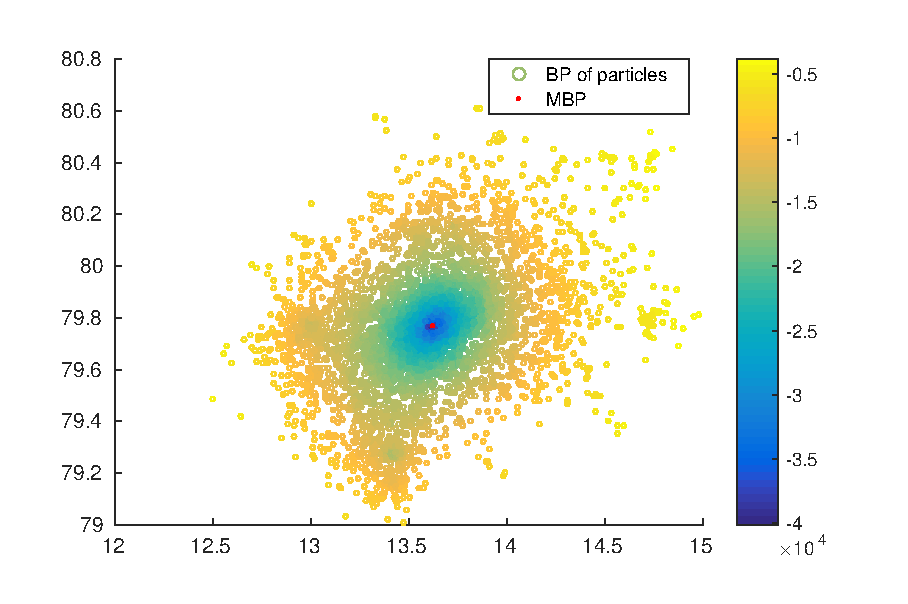
\includegraphics[scale=0.45]{naive}%
\caption{MBP Illustration}
\label{fig:naive}
\end{figure}
 \begin{algorithm}
\caption{Mixed Particle/Super-particle Hierarchy}
\label{sp-mixed}
\begin{algorithmic}[1]
\Procedure {$MBP=mixed\_kmeans(X,m)$}{}
\State $[IDX,c]=kmeans(X,N_c)$, where $N_c$ is  the number of clusters, $IDX\in \mathbb{N}^{N_p}$ is the index function to indicate which cluster particle $X_i$ belongs to, ${\bf c} _i \in \R^{2}, \, i=1,\dots,N_c$ is the centroid of each cluster. 
\State $\bar m_i=|\{j | IDX(j)=i\}|,\,\forall i=1:N_c$
\State $SBP_i=\ds\sum_{\{j|IDX(i)\neq j\}}\frac{\bar m_j}{d(X_i,c_j)}+\ds\sum_{\{j|IDX(j)=IDX(i),i\neq j\}}\frac{m_j}{d(X_i,X_j)},\, \forall i$ 
\State $MBP=\ds\min_i SBP_i$
\EndProcedure
\end{algorithmic} 
 \end{algorithm}
\begin{figure*}[t!]
\centering
\begin{subfigure}[t]{0.5\textwidth}
\centering
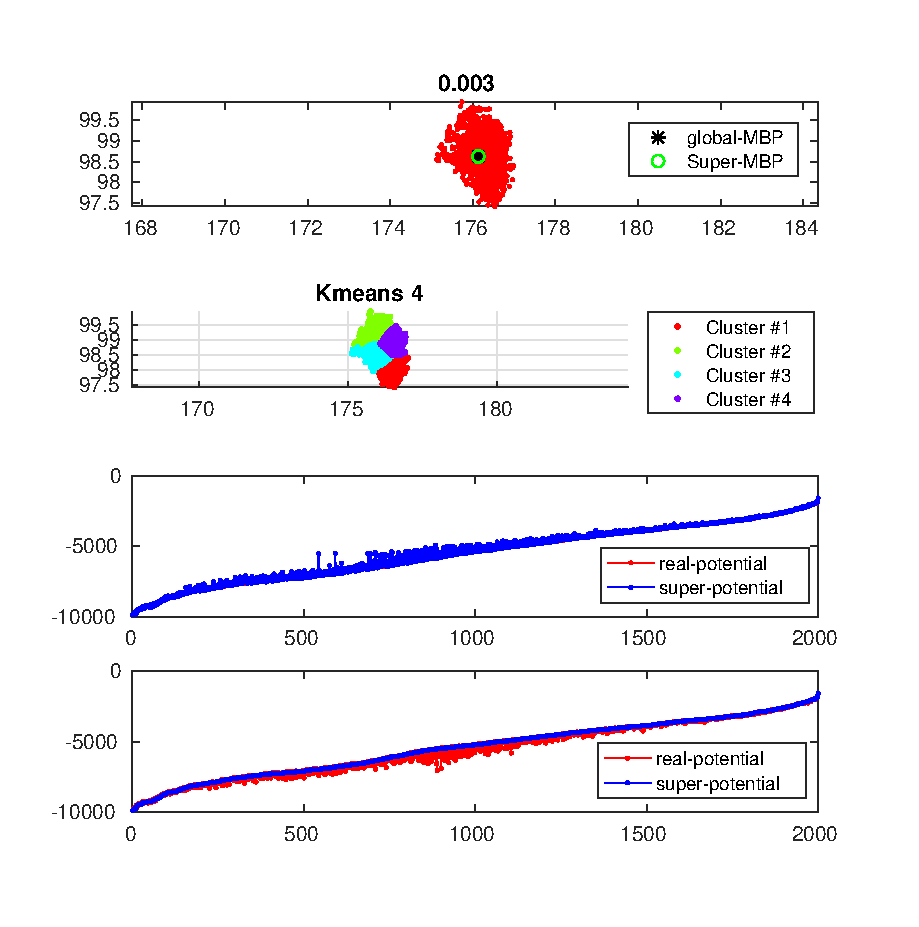
\includegraphics[scale=0.45]{sp_p_mixed_kmeans}
\end{subfigure}%
~ 
\begin{subfigure}[t]{0.5\textwidth}
\centering
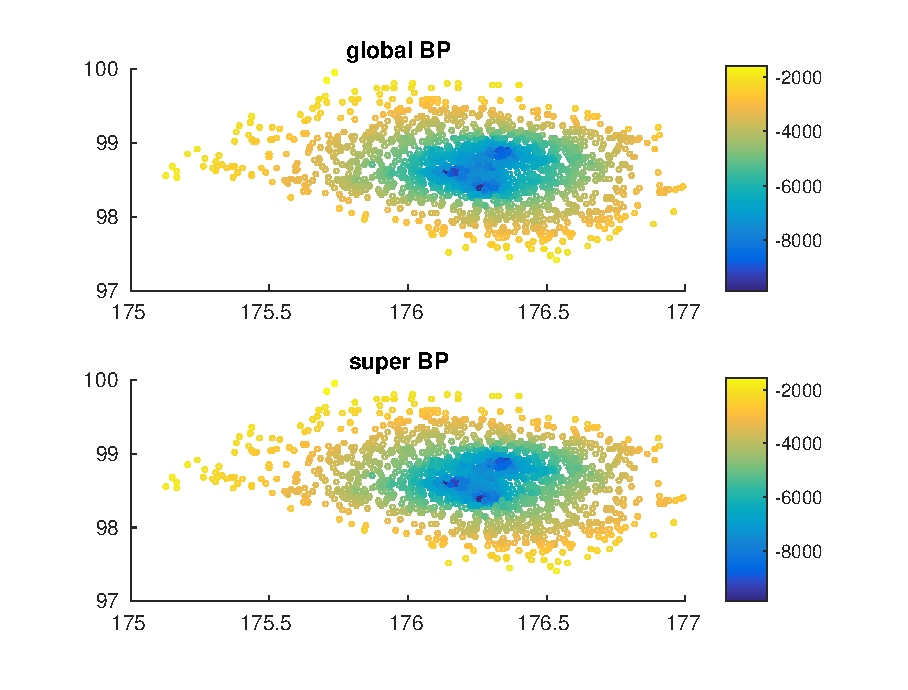
\includegraphics[scale=0.45]{sp_p_mixed_kmeans_bp}
\end{subfigure}
\caption{Result of Algorithm \ref{sp-mixed}}
\end{figure*}

 \begin{algorithm}
\caption{Super-particle Hierarchy}
\label{sp-p}
\begin{algorithmic}[1]
\Procedure {$MBP=sp\_kmeans(X,m)$}{}
\State $[IDX,c]=kmeans(X,N_c)$ 
\State $\bar m_i=|\{j | IDX(j)=i\}|,\,\forall i=1:N_c$
\State $MBP=\ds\min_i \ds\sum_{\{j|IDX(i)\neq j\}}\frac{\bar m_j}{d(X_i,c_j)}$ 
\State $n_c=N_c$
\State $k=1$
\While{$k\leq n_k$}
\State $MBP_{old} = MBP$
\State $v=\{j\,|\,IDX(j)=IDX(MBP)\}$
\State $[\tilde{IDX},\tilde{c}]=kmeans(X(i),\tilde{N_c}$
\State $c=\{c_1,\dots,c_{MBP-1}\}\cup\tilde{c}_1 \cup \{c_{MBP+1},\dots,c_{N_c}\}\cup \{\tilde{c}_2,\dots,\tilde{c}_{\tilde{N_c}}\}\}$
\State $IDX(v)=\tilde{IDX}+kN_c-1$
\State $n_c=n_c-1+\tilde{N_c}$
\State $\bar m_i=\frac{1}{|\{j | IDX(j)=i\}|},\,\forall i=1:n_c$
\State $MBP=\ds\min_i \ds\sum_{\{j|IDX(i)\neq j\}}\frac{\bar m_j}{d(X_i,c_j)}$ 
\If{$MBP=MBP_{old}$}
\State Stop
\EndIf
\State $k=k+1$
\EndWhile
\EndProcedure
\end{algorithmic} 
 \end{algorithm}
\begin{figure*}[t!]
\centering
\begin{subfigure}[t]{0.5\textwidth}
\centering
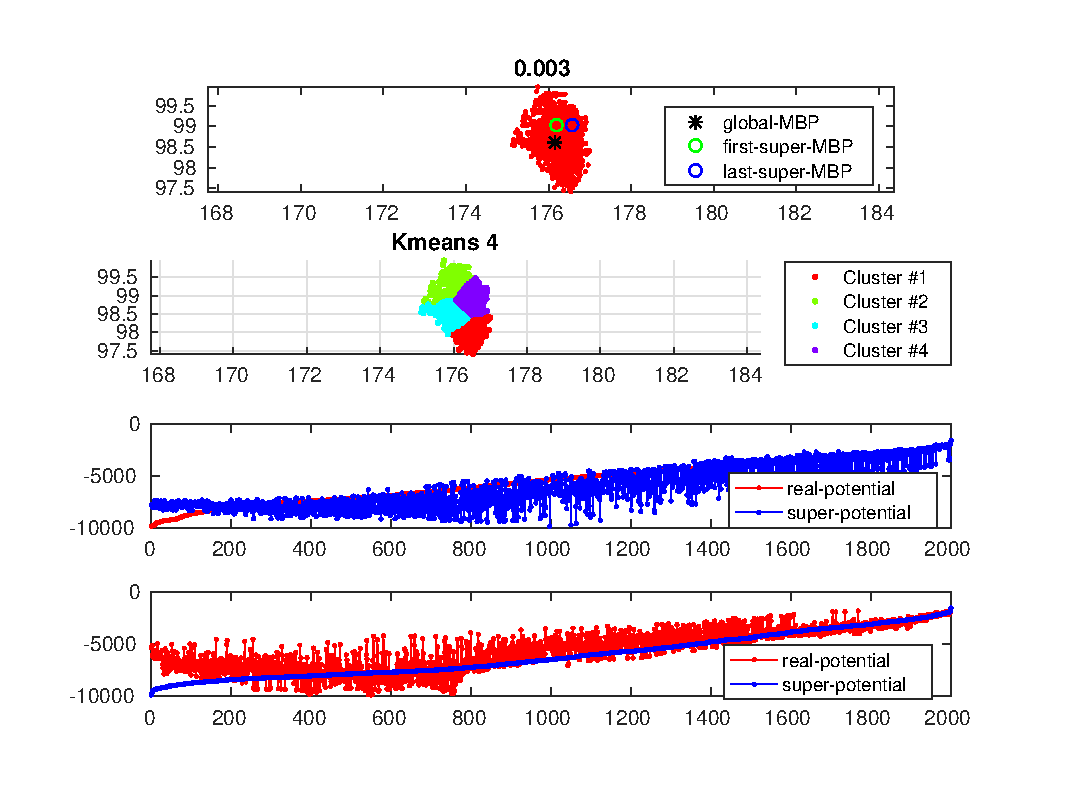
\includegraphics[scale=0.45]{sp_p_kmeans}
\end{subfigure}%
~ 
\begin{subfigure}[t]{0.5\textwidth}
\centering
\includegraphics[scale=0.45]{sp_p_kmeans_bp}
\end{subfigure}
\caption{Result of Algorithm \ref{sp-p}}
\end{figure*}
\begin{figure}[h]
\centering
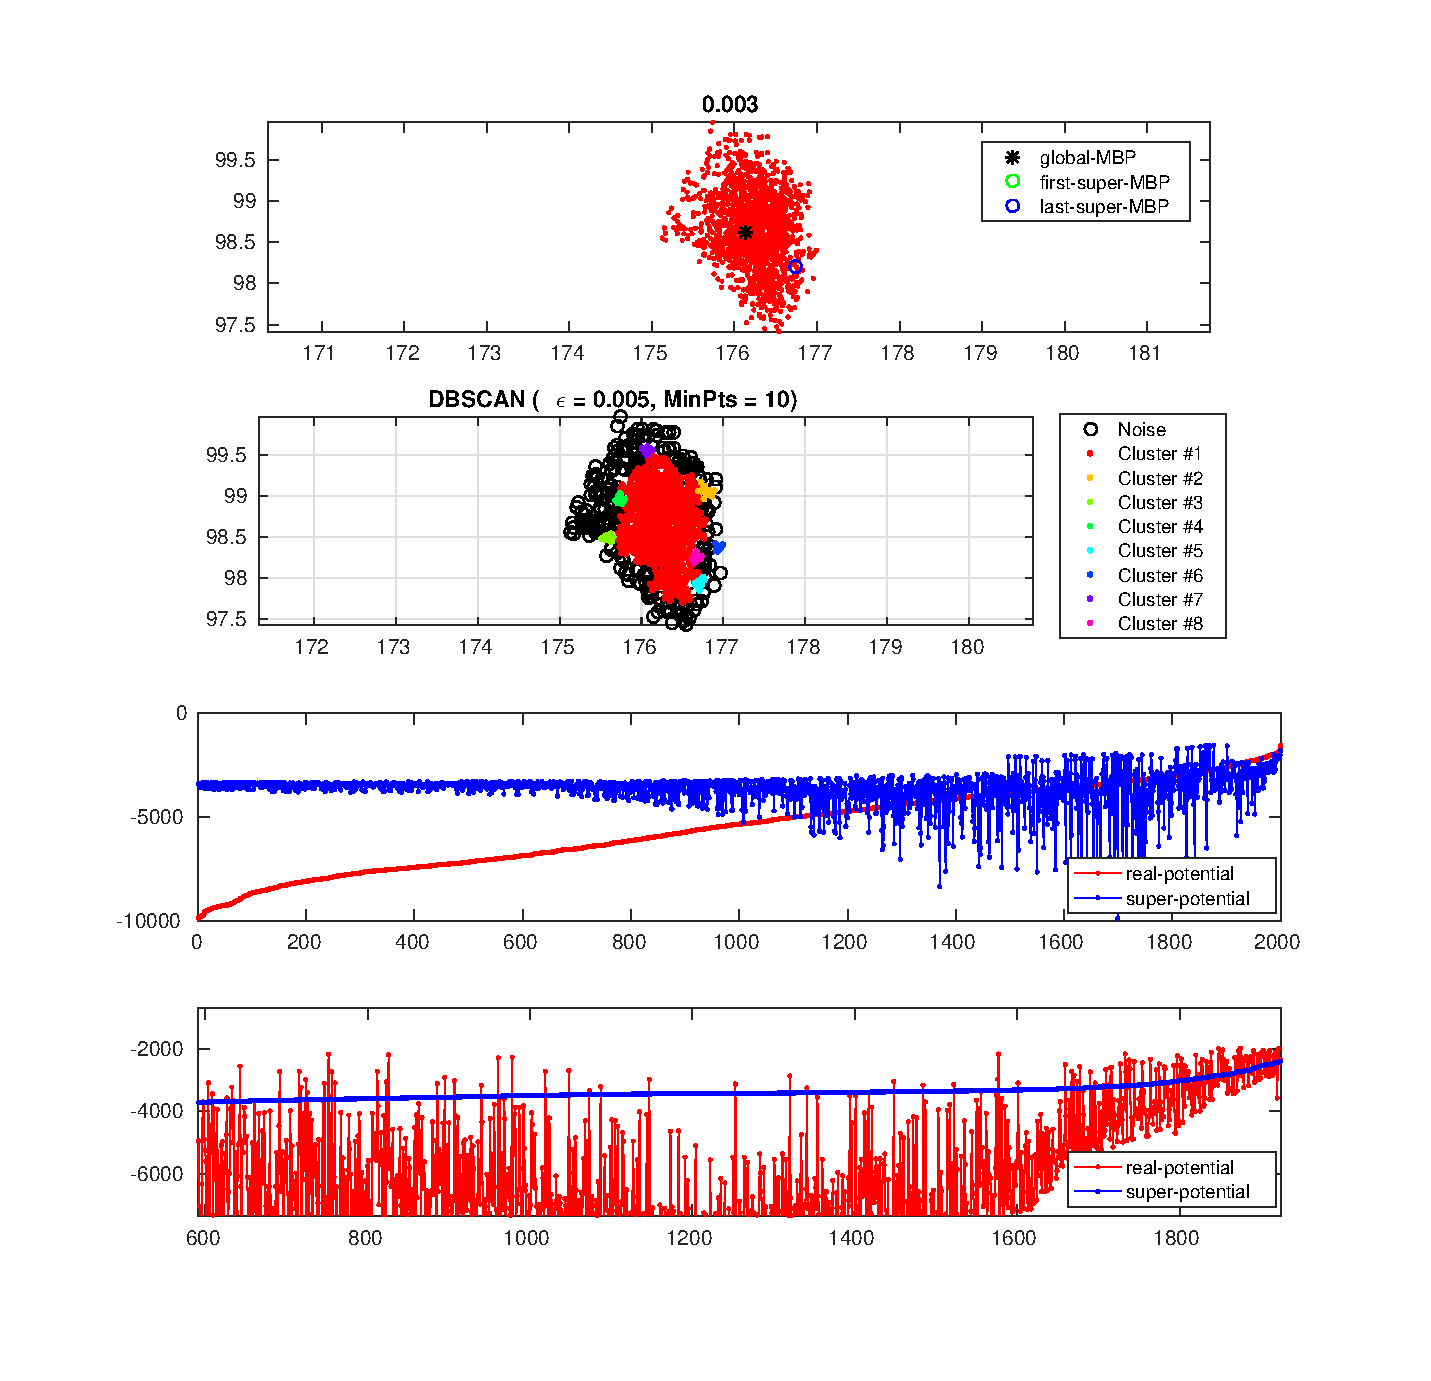
\includegraphics[scale=0.45]{sp_p_dbscan}%
\caption{Result of replacing Kmeans by DBSCAN in Algorithm \ref{sp-p}}
\label{fig:sp_dbscan}
\end{figure}

 \begin{algorithm}
\caption{Locate MBP from a subset of particles which forms the most dense super-particle via DBSCAN}
\label{dbscan_max}
\begin{algorithmic}[1]
\Procedure {$MBP=mbp\_dbscan\_max(X,m)$}{}
\State $[IDX,c]=dbscan(X,\varepsilon)$, where $\varepsilon$ is the linkage length provided for DBSCAN. 
\State $\bar m_i=|\{j | IDX(j)=i\}|,\,\forall i=1:N_c$, where $N_c$ is the resulted number of clusters given $\varepsilon$
\State $i_s=\ds\max_i \bar{m_i}$
\State $V=\{j \,|\, IDX(j)=i_s\}$
\State $SBP_i=\ds\sum_{i\neq j\}}\frac{m_j}{d(X_i,X_j)},\, \forall i\in V$ 
\State $MBP=\ds\min_{i\in V} SBP_i$
\EndProcedure
\end{algorithmic} 
 \end{algorithm}
\begin{figure}[H]
\centering
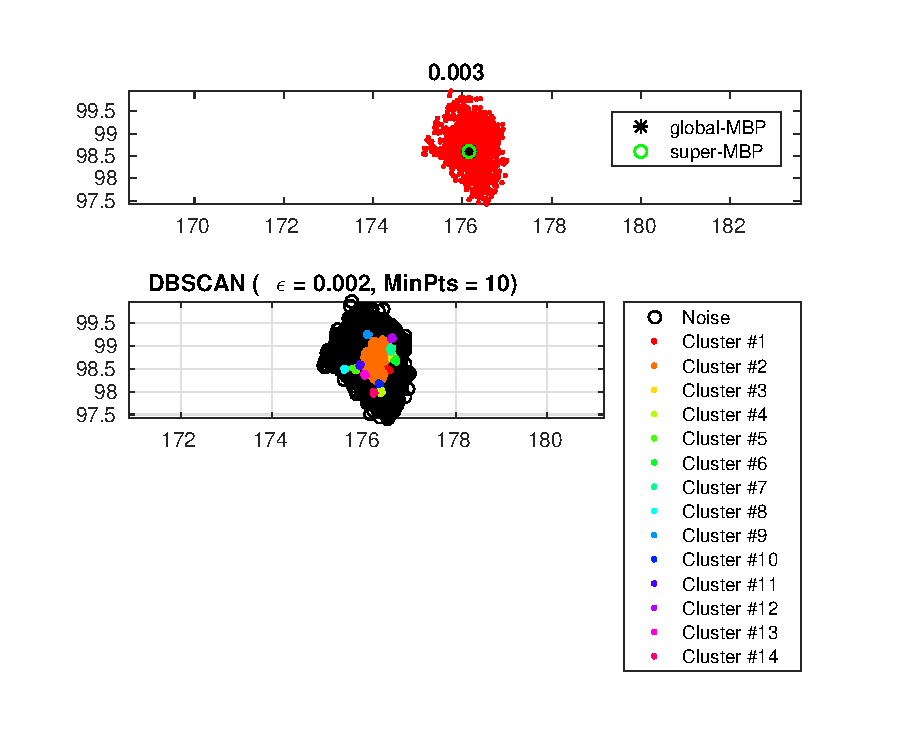
\includegraphics[scale=0.45]{p_dbscan_maxSub}%
\caption{Result of Algorithm \ref{dbscan_max}}
\label{fig:dbscan_max}
\end{figure}

